\section{Implementation}
\subsection{Grids}
In the implementation, we introduced a concept called grid. A grid was a visual representation of an area (any area) divided into discrete valued cells. The purpose of the grid was to easily view the actual situation and the predicted situation after reconstructing it based on samples from the actual situation (mobile phone sensor readings). As figure \ref{fig:grid-concept} shows, we used two separate grids placed next to each other where the left grid is always the actual situation and the right grid is always the predicted situation. These two grids served as a guide line throughout the implementation. If the grids did not look somewhat similar at all times, some error had been done. How these grids were used are explained in the following sections.

\begin{figure}[here]
\centering
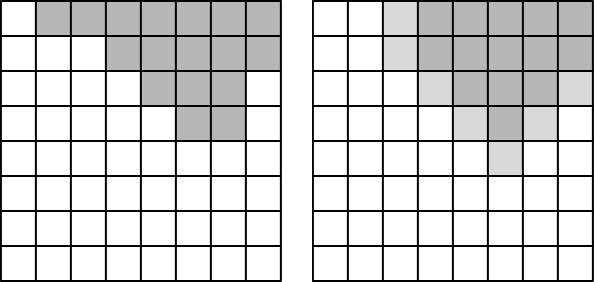
\includegraphics[width=0.5\textwidth]{solution/graphics/grid-concept.png}
\caption{Two grids are used to compare actual situation on the left and the estimated situation on the right.}
\label{fig:grid-concept}
\end{figure}

\subsection{Simulating Data}
Simulating data was done in the left grid. At launch, the user had to choose a location for the initial fire. A user could start several fires at once, where each one would spread independent of the other fires. The spreading was done automatically for each time iteration.

The fire spread was implemented with a simple algorithm. Given a two-dimensional grid of cells, the more burning neighbours each cell C on the grid had, the higher the chances were for it to ignite. Because there is a maximum of eight neighbors, we divided the number of burning neighbors by the total number of neighbors as shown in figure \ref{fig:fire-probability}.

\begin{figure}[here]
\centering
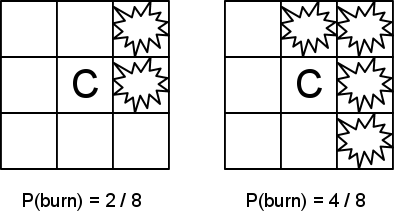
\includegraphics[width=0.5\textwidth]{solution/graphics/fire-probability.png}
\caption{Probability that fire will spread to a cell C on the grid without fire.}
\label{fig:fire-probability}
\end{figure}

The simple probability calculation was later extended to account for wind. Since wind can blow away smoke and heat wind direction and magnitude directly affects how much impact each neighboring cell would have on C. To simulate this, each neighboring cell used a portion of the wind vector to produce a weight of impact. The sum of all these weights divided by a total weight became the new probability calculation in the fire spreading algorithm.

Humidity was implemented after wind. Humidity affects how fast fire spreads. It was implemented as a global value and had the same value for each cell. With this simplicity, we only had to either increase or decrease the total weight used in the probability calculation to adjust the rate of fire spread.
\subsection{Sensing Data}
After simulating data with wind and humidity, the next step was to use mobile phone sensors to read this data. Even if the current situation was known through the simulation at all times, we were only supposed to know the situation by the mobile phone sensor readings. To simulate sensing, two additional algorithms were used.

The first algorithm was a walking algorithm to simulate that people walk around with the mobile phone sensors. This algorithm assumed that sensors already had a position in order to do the following. For each time step, there was a fifty percent chance for each sensor to move. Because there were eight different directions to walk in a grid, the sensor picked a random direction. If the neighboring cell in the picked direction was on fire, the sensor had to pick another direction. In all, this algorithm only handled the location of the mobile phone sensors in the simulation. The next step after placing the sensors was to do readings.

The second algorithm was a sensing algorithm to provide known data used by the crisis mapping system. Because heat and smoke moves in the direction of the wind, the resulting sensor readings highly depended on wind and the location of the fire. Consider the example in figure \ref{fig:sense-concept}. Given the same wind vector W and two different neighbors at relative positions V1 and V2, each neighbor contributes differently to the sensor in C. In this particular case, the wind either blow heat and smoke away from C or into C depending on which neighbor it is.

\begin{figure}[here]
\centering
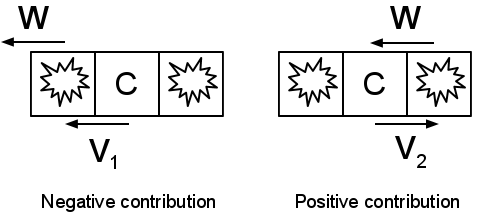
\includegraphics[width=0.65\textwidth]{solution/graphics/sense-concept.png}
\caption{Sensor readings are affected by wind and the positions of the neighboring emitting cells.}
\label{fig:sense-concept}
\end{figure}

The heat and smoke contribution to the sensor at C could be calculated as the sum of the cosine value of the angle between the wind vector W and the position vector for each neighbor. As shown in figure \ref{fig:sensor-contribution}, the cosine value could be divided into two ranges.

\begin{figure}[here]
\centering

\includegraphics[width=0.65\textwidth]{solution/graphics/sensor-contribution.png}
\caption{Neighbor heat and smoke contribution is found by the cosine value between on wind W and neighbor position V relative to the sensor.}
\label{fig:sensor-contribution}
\end{figure}

The range [-1,0] was equal to positive contribution while the remaining [0,1] was equal to negative contribution. In case of a negative contribution, the contribution can simply be treated as 0 because heat and smoke would blow away from the sensor. To further simplify, by taking the absolute value of the positive contribution range [-1,0], the new range became [0,1] where 0 is the lowest and 1 is the highest contribution. This could be used as a coefficient to the heat and smoke emitted by this neighbor. Given that there are eight neighbors each indexed by i, the resulting mathematical formula used in the sensing algorithm is as follows:

\[
  c = \sum_{\substack i=1}^8\left\{
  \begin{array}{l l}
    |V_i \cdot W / \left(|V_i | \cdot |W| \right)| & \quad \text{if $V_i \cdot W < 0$}\\
   0 & \quad \text{if $V_i \cdot W >= 0$}\\
  \end{array} \right.
\]
